\documentclass{beamer}
\usetheme{metropolis}

\usetheme{metropolis}
\usepackage{listings}

\lstdefinestyle{Python}
{
    language=Python,
    basicstyle=\ttfamily\scriptsize,
    keywordstyle=\color{blue}\ttfamily,
	otherkeywords={self,False},
    commentstyle=\color{green!60!black}\ttfamily,
    stringstyle=\color{red!80!black}\ttfamily,
    backgroundcolor=\color{blue!10!white},
    showstringspaces=false,
    numbers=none,
    numberstyle=\tiny,
    numbersep=5pt,
    xleftmargin=2pt,
    framexleftmargin=4pt,
    framexrightmargin=4pt,
    framexbottommargin=5pt,
    framextopmargin=5pt,
    %breaklines=true,
    captionpos=b
}

\lstdefinestyle{MATLAB}{
    language=MATLAB,
    basicstyle=\ttfamily\scriptsize,
    keywordstyle=\color{blue}\ttfamily,
    stringstyle=\color{red!80!black}\ttfamily,
    commentstyle=\color{green!60!black}\ttfamily,
    numbers=none,
    backgroundcolor=\color{orange!15!white},
    showstringspaces=false,
    numbers=none,
    numberstyle=\tiny,
    numbersep=5pt,
    xleftmargin=2pt,
    framexleftmargin=4pt,
    framexrightmargin=4pt,
    framexbottommargin=5pt,
    framextopmargin=5pt,
    %breaklines=true,
    captionpos=b
}

\renewcommand{\emph}[1]{{\color{red}#1}}

\beamerdefaultoverlayspecification{<+->}

\setbeamercolor{block body}{bg=mDarkTeal!30}
\setbeamercolor{block title}{bg=mDarkTeal,fg=black!2}

\title{Test-Driven Development}
\author{Joachim Vandekerckhove}
\date{}


\newcommand{\module}[1]{{\color{brown}\texttt{#1}}}
\newcommand{\code}[1]{{\color{blue}\texttt{#1}}}

\title{Simulation}
\author{Joachim Vandekerckhove}
\date{}

\usepackage{graphicx}
\begin{document}


\title{Static versus instance methods}
\begin{frame}
  \maketitle
\end{frame}

\begin{frame}[fragile]{Static Methods}
    A static method is a method that \emph{belongs to the class itself} rather than to a particular instance of the class. Here's an example of how to define a static method in MATLAB:
    \begin{lstlisting}[style=Matlab]
    classdef MyClass
        methods (Static)
            function out = my_static_method(arg1, arg2)
                % Code for static method goes here
            end
        end
    end
    \end{lstlisting}
    To call a static method in MATLAB, you can use the class name followed by the method name, like this:
    \begin{lstlisting}[style=Matlab]
    MyClass.my_static_method(arg1, arg2)
    \end{lstlisting}
\end{frame}

\begin{frame}[fragile]{When to Use Static Methods}
    Static methods cannot access instance variables or methods, since they don't have access to a particular instance of the class. If you need to access instance variables or methods, use a regular instance method instead.
    
    Static methods are useful:
    \begin{itemize}
        \item When a method doesn't need to access any instance variables or methods of the class
        \item When a method needs to be called from both the class and instances of the class
        \item When a method is not logically tied to any particular instance of the class
        \item To create specialized instances of the class
    \end{itemize}
\end{frame}

\begin{frame}[fragile]{Static Factory Method}
    A static factory method creates an instance:
    \begin{lstlisting}[style=Matlab]
    classdef BankAccount
        properties
            balance = 0;
        end
        methods
            function obj = BankAccount(balance)
                obj.balance = balance; end
        end
        methods (Static)
            function obj = create_empty_account()
                obj = BankAccount(0); end
            function obj = load(filename)
                saved = load(filename); obj = saved.obj; end
        end
    end
    \end{lstlisting}
    Now you can create basic instances of \code{BankAccount}:
    \begin{lstlisting}[style=Matlab]
    account = BankAccount.create_empty_account();
    \end{lstlisting}
\end{frame}






\title{Simulation}
\begin{frame}
  \maketitle
\end{frame}

\begin{frame}[fragile]{Random Number Generation: Overview of Algorithms}
    Random number generation is the process of generating a sequence of numbers that are not predictable and have no discernible pattern. There are many algorithms for generating random numbers, but they can be broadly classified into two categories:
    \begin{itemize}
        \item Pseudorandom number generators: These are algorithms that use a deterministic process to generate a sequence of numbers that appear random, but are actually predictable if you know the algorithm and the seed value that was used to initialize it.
        \item True random number generators: These are algorithms that generate numbers from a source of entropy, such as atmospheric noise or radioactive decay, that are truly random and not predictable.
    \end{itemize}
\end{frame}

\begin{frame}[fragile]{Generating Random Numbers in MATLAB}

The \code{rand()} function in MATLAB generates a random float between 0 and 1.

\begin{lstlisting}[style=matlab]
n = rand();
disp(n)  % prints a random float between 0 and 1
\end{lstlisting}

\end{frame}

\begin{frame}[fragile]{Seeding Random Number Generators}
    Pseudorandom number generators use a \emph{seed value} to initialize the algorithm. If you use the same seed value, you will get the same sequence of numbers every time:

\begin{lstlisting}[style=matlab]
rng(1234)  % seed with a fixed value
n = rand();
disp(n)  % prints 0.1915
\end{lstlisting}

By using the same seed value, we can ensure that the same random sequence is generated every time the code is run.

Note: MATLAB starts up with a default seed!

\end{frame}

\begin{frame}[fragile]{Sampling from Statistical Distributions}
The \code{normrnd()} function in MATLAB generates random variables from a Gaussian distribution with the specified mean and standard deviation:

\begin{lstlisting}[style=matlab]
mu    = 0;  % Gaussian mean
sigma = 1;  % Gaussian standard deviation

n = normrnd(mu, sigma);
\end{lstlisting}

\end{frame}


\begin{frame}[fragile]{More examples}

Generate a sequence of 5 random integers from a binomial distribution with 10 trials and probability of success 0.5
    \begin{lstlisting}[style=matlab]
b = binornd(10, 0.5, 5, 1);
    \end{lstlisting}

Generate 10 numbers from a standard uniform distribution
    \begin{lstlisting}[style=matlab]
n = rand(10, 1);
    \end{lstlisting}

Generate 10 integers from a discrete uniform between 1 and 100
    \begin{lstlisting}[style=matlab]
du = randi([1, 100], 10, 1);
    \end{lstlisting}
    
Generate SDT data from 100 signal and 10 noise trials
    \begin{lstlisting}[style=matlab]
hr = 0.6; far = 0.4; nSig = 100; nNoi = 10;
hits = binornd(nSig, hr);
fas  = binornd(nNoi, far);
    \end{lstlisting}

\end{frame}





\begin{frame}{Diffusion Model Sampling}
The diffusion model is a popular cognitive model that describes decision-making processes. In this model, decision-making is represented as a diffusion process of evidence accumulation.

The model assumes that a decision is made by accumulating evidence in favor of one of two alternatives, and that the evidence is accumulated continuously over time until a decision boundary is reached.
\end{frame}


\begin{frame}{Diffusion Model Sampling}
\begin{figure}[htp]
\centering
\includegraphics[scale=0.7]{wdm.eps}
\caption{The Wiener diffusion model}
\label{}
\end{figure}
\end{frame}


\begin{frame}{Euler-Maruyama Method}

\textbf{Idea:} Approximate the continuous-time process $X(t)$ using a discrete-time approximation $X_n = X(n \Delta t)$, where $\Delta t$ is the time step size.

\pause

\begin{block}{Euler-Maruyama Method}
    Given the SDE: 
    $$ dX(t) = f(X(t), t) dt + g(X(t), t) dW(t), $$
    with $X(0) = x_0$, the Euler-Maruyama method generates a numerical approximation $X_n$ for $X(n\Delta t)$ via the recursion: 
    $$ X_{n+1} = X_n + f(X_n, n\Delta t) \Delta t + g(X_n, n\Delta t) \Delta W_n,$$
    where $\Delta W_n = W_{(n+1)\Delta t} - W_{n\Delta t}$ and $W_t$ is the Wiener process.
\end{block}

\end{frame}



\begin{frame}{Diffusion Model Sampling}

To simulate the diffusion process, we can use the following equations:
\begin{align*}
dx_t &= \delta dt + \sigma dW_t \\
x_t &= x_{t-1} + dx_t
\end{align*}

where $x_t$ is the evidence at time $t$, $\delta$ is the drift rate, $\sigma$ is the diffusion coefficient, $dW_t$ is a Wiener process (i.e., a random noise process), and $dt$ is a small time step.

\end{frame}


\begin{frame}[fragile]{Diffusion Model Sampling}

Simulate the diffusion process using MATLAB:

\begin{lstlisting}[style=Matlab]
dt    = 0.001;
T     = 1.0;
mu    = 0.1;
sigma = 0.5;
y0    = 0.0;

% Initialize and preallocate arrays
t   = 0:dt:T;
y   = zeros(size(t)) + y0;
rnd = randn(size(t));

% Simulate diffusion process
for i = 2:length(t)
    dy = mu * dt + sigma * sqrt(dt) * rnd(i);
    y(i) = y(i-1) + dy;
end
\end{lstlisting}


\end{frame}


\begin{frame}[fragile]{Diffusion Model Sampling}
\begin{figure}[htp]
\centering
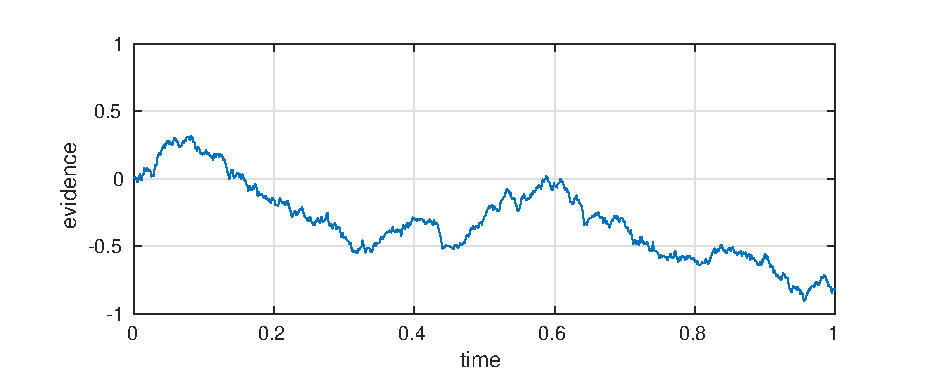
\includegraphics[scale=0.7]{diff.eps}
\caption{A single diffusion process}
\label{}
\end{figure}
\end{frame}






\end{document}

% Static methods
% Random number generation
% - Streams
% Simulating data


% HW:
% - Simulate SDT data
% - ROC Curve
% - Fit ROC curve?
% - Fit line?